% article,book,report
% ctexart,ctexbook,ctexreport 中文
\documentclass[UTF8,AutoFakeBold]{ctexart}
%! 请使用XeLaTex 进行排版
%! 需要编译两次,才能更新 TOC 哦


\usepackage[]{color}

\usepackage{graphicx}     % 插入图片的宏包
\usepackage{float}        % 设置图片浮动位置的宏包
\usepackage{subfigure}    % 插入多图时用子图显示的宏包
\usepackage{listings}     % 代码
\usepackage{xcolor}       % 代码高亮

\usepackage{geometry}     % 设置边距
\usepackage{verbatim}     % 显示原始字符
\usepackage{cprotect}     % 在标题中显示原始字符
\usepackage{ulem}         % 删除

\usepackage{amsmath}      % 图表添加章节编号

% \usepackage[colorlinks=true]{hyperref}
\usepackage{hyperref}




% checkbox
\usepackage{bbding}
\usepackage{pifont}
\usepackage{wasysym}
\usepackage{amssymb}


%**********************边距设置****************************************

% \geometry{a4paper,scale=0.8}
\geometry{a4paper,left=2cm,right=2cm,top=2cm,bottom=2cm}

%********************代码设置******************************************
% 用来设置附录中代码的样式

\lstset{
    backgroundcolor     =   \color[RGB]{250,240,235},
    basicstyle          =   \zihao{5}\ttfamily,                % sf/tt基本代码风格
    keywordstyle        =   \bfseries,                % 关键字风格
    commentstyle        =   \rmfamily\itshape,        % 注释的风格,斜体
    stringstyle         =   \ttfamily,                % 字符串风格
    flexiblecolumns,                                  % 别问为什么,加上这个
    numbers             =   left,                     % 行号的位置在左边
    showspaces          =   false,                    % 是否显示空格,显示了有点乱,所以不现实了
    numberstyle         =   \zihao{-5}\ttfamily,      % 行号的样式,小五号,tt等宽字体
    showstringspaces    =   false,
    captionpos          =   t,                        % 这段代码的名字所呈现的位置,t指的是top上面
    frame               =  ltb,% lrtb,                     % 显示边框
    breaklines          =  true,
}

\lstdefinestyle{Python}{
    language        =   Python,                       % 语言选Python
    basicstyle      =   \zihao{-5}\ttfamily,
    numberstyle     =   \zihao{-5}\ttfamily,
    keywordstyle    =   \color{blue},
    keywordstyle    =   [2] \color{teal},
    stringstyle     =   \color{magenta},
    commentstyle    =   \color{red}\ttfamily,
    breaklines      =   true,                         % 自动换行,建议不要写太长的行
    columns         =   fixed,                        % 如果不加这一句,字间距就不固定,很丑,必须加
    basewidth       =   0.5em,
}

%*************** 超链接设置***************
\hypersetup{
    colorlinks  = true,
    linkcolor   = blue,
    filecolor   = magenta,
    urlcolor    = cyan,
    % pdftitle    = {Overleaf Example},
    % pdfpagemode = FullScreen,
}
%**Latex技巧:在图表序号中加入章节号(实现诸如“图1.1.2”这样的图表序号)*******************************
% https://blog.csdn.net/Canhui_WANG/article/details/87364800
\numberwithin{figure}{section}
\numberwithin{table}{section}

%****************************
\begin{document}
\title{\LaTeX 入门手册}
\author{$\heartsuit$Liuding.xin$\heartsuit$}
\date{2021-05-20}


% 标题
\begin{titlepage}
    \maketitle %将title 编译进来
    % todo 想知道如何设置为背景图
    \begin{figure}[htbp]
        \centering
        
\includegraphics[scale=0.4,angle=-50]{images/1200px_LaTeX_project_logo_bird.svg.png}
    \end{figure}
\end{titlepage}

% 本文的目录
\tableofcontents

%图标的目录
\listoffigures

%表格的目录
\listoftables

\clearpage

\begin{abstract}
    本文是记录在学习\LaTeX 过程中遇到的问题和解决办法,并用\LaTeX 写出来。

    真的好困难。希望大家在看到这个文档的时候,点个赞!$\heartsuit$$\heartsuit$$\heartsuit$
\end{abstract}

\section{\LaTeX 基础}
\label{sec:knowledge}

\subsection{什么是\LaTeX?}
TeX 是高老师编写的非常流行的排版软件。\LaTeX 是基于 Tex 之后,集合更多宏包的再发行版本。\LaTeX 更加简单更流行,但是还是很难入门,因为他们都是使用markup语言进行编写,而不是类似 $MicroSoft Word$ 那样所见即所得。所以门槛非常高。
但是一旦学习并熟悉,对论文的编写是非常有用的。尤其是他的模板功能。而且任何东西都是可以细粒的控制的。正是因为门槛很高,导致学习非常陡峭,让很多人想入手都不知道如何入手。

本人也是折腾了很久之后,终于找到了学习方法和技巧。后续将会简单的给大家讲解如何上手。

这里将会讲解非常简单的基础。

当然入手难的问题实在是要靠自己去解决,所以不要认为最好的排版软件就是最适合自己的。你可以根据自己的需求选择不同的排版软件。

比如:
\begin{enumerate}
    \item $Micro$ $Soft$ $Word$.
    \item \LaTeX
    \item $Markdown$
\end{enumerate}

但是如何选择可以参考:

\Checkmark 选择使用 TEX/LATEX 的理由包括:

\begin{itemize}
    \item 免费软件;
    \item 专业的排版效果;
    \item 是事实上的专业数学排版标准;
    \item 广泛的西文期刊接收甚或只接收 LaTeX 格式的投稿;
\end{itemize}

\Checkmark 不选择使用 TEX/LATEX 的理由包括:
\begin{itemize}
    \item 需要相当精力学习;
    \item 图文混合排版能力弱;
    \item 仅流行于数学、物理、计算机等领域;
    \item 中文期刊的支持较差;
\end{itemize}

\subsection{如何查询文档?}
对于这种非常陌生羞涩难懂的软件。你会觉得连查文档都很困难。不过如果你想对某个模块阅读文档,可以通过下面的命令打开英文文档。

\begin{lstlisting}
> texdoc 模块的名字
> texdoc lstlisting
\end{lstlisting}


\subsection{\LaTeX 文类层级}
\label{sec:structure}
%定义一个跳转地址
\hypertarget{Levelofdepth}{\LaTeX} 有三种标准文类:book, report, article。中文是 ctexart。

每种文类的章节命令和层次深度如下:


\begin{table}[htbp]
    \centering
    \begin{tabular}{|c|c|c|c|c|}
        \hline
        层次深度 & 层次名        & book                      & report                    & article                   \\
        \hline
        -1       & part          & $\backslash$part          & $\backslash$part          &                           \\
        0        & chapter       & $\backslash$chapter       & $\backslash$chapter       & $\backslash$part          \\
        1        & section       & $\backslash$section       & $\backslash$section       & $\backslash$section       \\
        2        & subsection    & $\backslash$subsection    & $\backslash$subsection    & $\backslash$subsection    \\
        3        & subsubsection & $\backslash$subsubsection & $\backslash$subsubsection & $\backslash$subsubsection \\
        4        & paragraph     & $\backslash$paragraph     & $\backslash$paragraph     & $\backslash$paragraph     \\
        5        & subparagraph  & $\backslash$subparagraph  & $\backslash$subparagraph  & $\backslash$subparagraph  \\
        \hline
    \end{tabular}
    \caption{不同标准文类的章节命令与层次深度}
    \label{tab:typeoflatex}
\end{table}

\subsection{\LaTeX 编码问题}
% 引用一个跳转地址
上述 \hyperlink{Levelofdepth}{层次结构} 中, 我们知道有三类book, report, article,中文的article是ctexart。
但是如果我们需要在西文中插入中文要如何弄呢?
这就需要引用CKJ 包了。

\begin{enumerate}
    \item \Checkmark 引用包\verb!usepackage{CJK}!
    \item \Checkmark 在需要的写入中文的地方引用下面的代码。

          \begin{lstlisting}
\begin{CJK}{UTF8}{gbsn}
    你好
\end{CJK}
        \end{lstlisting}
    \item $\Box$ Why gbsn?
    \item $\Box$ What is the difference between CJK and CJK-utf8?
\end{enumerate}

% \subsection{\LaTeX 文档结构}
\subsection{\LaTeX 文档结构}
\subsubsection{\LaTeX 的编写思路}
要想写一个\LaTeX 的文档,其实很简单.

\LaTeX 主要分为三部分。可以理解为我要写什么,我要开始写文档,我正在写文档.
\begin{enumerate}
    \item  说明我要写说明文档,就是我要写什么;

          \begin{verbatim}
% cjk 使用utf-8,中文文章使用`ctexart`,article,report,...
% 大意就是说我要写什么
\documentclass[UTF8]{ctexart}
        \end{verbatim}
    \item  说明我要用到的宏包,就是我要开始写;

          \begin{verbatim}
% 宏包,意思是我要开始写文档了。我会用什么工具。只有加了宏包才能写公式,做表格,放图片
% 常用的有mathtools,amsmath,graphicx,array,geometry
\usepackage{mathtools,booktabs}
        \end{verbatim}
    \item  说明我要用到的环境,就是我正在写.

          \begin{verbatim}
% 这里是导言区
\begin{document}% 这是一个文档的环境
    document
    \begin{figure}% 这是一个图片的环境
        图片配置
    \end{figure}
    \begin{table}% 这是一个表格的环境
        表格代码
    \end{table}
\end{document}
        \end{verbatim}
\end{enumerate}


\subsubsection{\LaTeX 的文件类型}
\label{subsec:filetype}
\url{https://blog.csdn.net/huitailangyz/article/details/99685683}{VSCode 的配置过程}

tex: tex文件是最常见的latex文件,也是平时编写文章的文件

cls: cls文件是latex的格式文件,规定了tex源文件的排版格局,称为类文件(class)

一般使用\verb!\documentclass{}!导入

sty: sty文件是宏包文件(package)

一般使用\verb!\usepackage{}!导入

bst: bst文件是参考文件的格式文件

一般使用\verb!\bibliographystyle{}!导入

bib: bib文件是参考文献的库

一般使用\verb!\bibliography{}!导入

bib文件一般如下:
\begin{lstlisting}
    @article{XXX,
        title={ABC},
        author={A, B},
        journal={XX},
        year={20XX}
    }
    @inproceedings{YYY,
        title={ABC},
        author={A, B, C},
        booktitle={YY},
        pages={a--b},
        year={20YY}
    }
\end{lstlisting}

\subsubsection{\LaTeX 文件语法结构}

假设在当前目录下有下列文件:main.tex、A.cls、B.sty、C.bst、D.bib,按照我们的文件格式\ref{subsec:filetype}。我们可以大致的了解真正的\LaTeX 的语法结构。

\begin{lstlisting}
%main.tex文件
\documentclass{A}     % 或者不使用自定义的排版文件时,使用最普通的\documentclass{article}
\usepackage{B}        % 以及导入一些其他常用的宏文件,如amsmath、amssymb、amsthm等数学相关的宏文件
\begin{document}
XXX
XXX
XXX
% 正文结束
\bibliography{D}      % 导入正文中引入文献的数据
\bibliographystyle{C} % 导入参考文献的格式文件C.bst
\end{document}
\end{lstlisting}


\subsection{常用的工具和资源链接}

\subsubsection{一些入门网站}

入门书籍。建议先看: \href{https://github.com/heartacker/MyNotes/blob/master/01.Latex/LaTeX_Docs_2014/04%20%E7%94%B5%E5%AD%90%E4%B9%A6/LaTeX%E5%85%A5%E9%97%A8%EF%BC%88%E5%88%98%E6%B5%B7%E6%B4%8B%EF%BC%89.pdf}{LaTeX入门(刘海洋).pdf}

TexLive 安装: \href{https://zhuanlan.zhihu.com/p/136931926}{TexLive 2020 安装指南}

软件配置教程: \href{https://blog.csdn.net/qq_23599965/article/details/103022215}{用于 Visual Studio Code 的 LaTeX Workshop}

手写识别: \href{http://detexify.kirelabs.org/classify.html}{手写体符号识别工具}。

在线公式编辑器: \href{https://latexlive.com/}{在线\LaTeX 公式编辑器}, 支持导出多个格式。

插入代码: \href{https://zhuanlan.zhihu.com/p/65441079}{LaTeX 里「添加程序代码」的完美解决方案}

学习入门总结: \href{https://www.cnblogs.com/zyg123/p/10499744.html}{LaTeX学习系列之---LaTeX的总结}



\subsubsection{常用宏包}


常见的宏包推荐。
来源:\href{https://www.zhihu.com/question/26421957/answer/32801779}{zhihu\@ 孟晨}

首先是国外用户写的一篇文档。
\href{http://www.howtotex.com/packages/9-essential-latex-packages-everyone-should-use/}{9 essential LaTeX packages everyone should us},Elegant LaTeX Team 有翻译。


\textbf{中文支持。}

ctex - 封装好的中文支持和版式调整工具,定义了许多方便的工具

xeCJK - XeLaTeX 下的中文字体选择和禁则、压缩的处理

fontspec - XeLaTeX 下的西文字体选择


\textbf{页面布局类。}

geometry - 调整页面大小、页边距等尺寸

fancyhdr - 设计页眉页脚

titlesec - 设计章节标题格式

titletoc - 设计目录格式


\textbf{超链接和PDF 的各种功能。}

hyperref - 超链接,PDF 书签,PDF 表单,PDF 元信息……

media9 - 插入 Flash、视频等


\textbf{图表和浮动体。}

graphicx - 插图

xcolor - 颜色

tikz - 绘图

booktabs - 三线表

multirow - 列合并单元格(cell)

makecell - 在单元格内手动换行

longtable - 换页表格

tabu - 封装了各种接口的表格宏包,制表强烈推荐

threeparttable - 在表格中使用脚标,和 tabu 有冲突,补丁:https://gist.github.com/157a703e0ed8804e7696

diagbox - 斜线表头(作者: @刘海洋)

float - 提供了 H 选项,禁止浮动体浮动(除非必要,不建议这么干)

placeins - 提供了 \verb!\FloatBarrier! 命令,限制浮动体浮动范围

\textbf{列表环境。}

enumitem - 修改列表环境的各种间距、label 样式等的不二法门

\textbf{其他一些工具。}

nag - 检查你是否使用了过时的宏包和命令的宏包

etoolbox - 主要是针对宏包和文档类开发者,不过提供了一些对环境的钩子,有时候很有用

xpatch - 修补命令用的

environ - 增强了 LaTeX 本来的 \verb!\newenvironment!的功能,解决了一些花括号不匹配导致的问题

\newpage
% \section{\LaTeX 学习笔记}
\section{\LaTeX 学习笔记}
\label{sec:skillnotes}

在基础知识\ref{sec:knowledge}里面提到。


%*\subsection{如何生成目录?}
\subsection{如何生成目录?}
制作目录其实非常简单,只需要一个命令,就是 \verb!\tableofcontents! 。这个命令放在哪里,目录就会出现在哪里。和交叉引用相同的一个特点是,目录的排版也需要两次编译。一方面是因为其中涉及到页码,另一方面是涉及到各个章节的标题。

\subsubsection{内置目录}

\begin{quotation}
    Tip: 只要生成了目录,之后生成的PDF 就会包含书签。
\end{quotation}

目录对于图表而言也是可以用的。如果你的文档中有很多图表,也可以专门为它们建目录。对应的命令是 \verb!\listoffigures! 和 \verb!\listoftables! 。它会收集对应图表中的标题来产生图表的目录。图表的插入我们将在下一期中介绍。

注意,这会在目录下生成\verb!.toc!,\verb!.lof!, \verb!.lot!  文件,分别对应【目录】、【图像】、【表格】。

\begin{enumerate}
    \item 目录

          \verb!\tableofcontents!
    \item 图像

          \verb!\listoffigures!
    \item 表格

          \verb!\listoftables!
\end{enumerate}

不过,需要注意的是,在编译的时候,需要使用编译工具进行编译两次。第一次是初步编译,生成目录等临时文件,之后在将临时文件编译进去。比如第一次编译之后,生成的PDF文件是看不到目录的,之后再次编译,就可以把 .toc、.lof、.lot编译进去。


\subsubsection{如何对某个定义对象进行编号?}
% todo
如,代码,摘要,附录。
todo


\subsection{如何让标题单独一个封面?}

有些书籍封面是单独一个页面的,还配了图片。看起来非常舒服,这个该如何处理呢?可以参考以下代码:

\begin{lstlisting}
%标题
\begin{titlepage}
    \maketitle %将title 编译进来
    \centering
    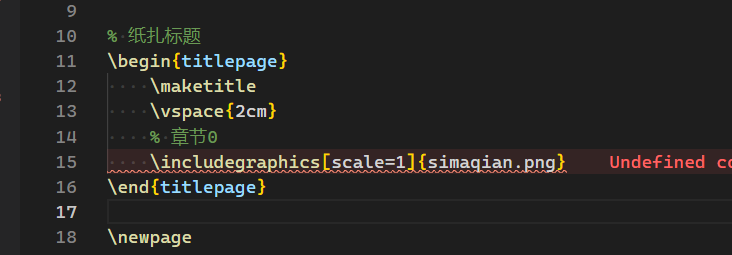
\includegraphics[scale=1.5]{simaqian.png} % 顺便插入图片
\end{titlepage}
\end{lstlisting}


\subsection{基础字体样式调节}

\subsubsection{常用样式}

\emph{Italicized text} 斜体使用\verb!\emph{Italicized text}! 进行标记。

\textbf{Bold text} 粗体使用\verb!\textbf{Bold text}! 进行标记。

\underline{Underlined text} 下划线使用\verb!\underline{Underlined text}! 进行标记。

\textit{Emphasising text} 强调使用\verb!\textit{Emphasising text}! 进行标记。

\textbf{\textit{Combine text} \underline{当然也可以组合起来}},\verb!\textbf{\textit{combine text}! 进行标记。

\subsubsection{中文的加粗}
也不知道什么原因,参考,\href{https://www.zhihu.com/question/58456658}{xelatex编译加粗楷体为什么会失败?} 默认情况下,使用 \verb!\textbf{加粗}! 是不会加粗的。处理方法是,在启用 \verb!AutoFakeBold!。
比如:
\begin{lstlisting}
% 在class 里面启用 AutoFakeBold
\documentclass[UTF8,AutoFakeBold]{ctexart}

% 或者

\end{lstlisting}



\subsubsection{删除线}
删除线比较复杂, 但是需要引用ulem的宏包。
\begin{enumerate}


    \item \verb!\usepackage{ulem}!;

    \item 使用方法:
          \begin{lstlisting}
\sout{文字}   %删除线
\uwave{文字}  %波浪线
\xout{文字}   %斜删除线
\uuline{文字} %双下划线
\end{lstlisting}

    \item 显示效果:
          \begin{enumerate}
              \item \sout{删除线}   %删除线
              \item \uwave{波浪线}  %波浪线
              \item \xout{斜删除线}   %斜删除线
              \item \uuline{双下划线} %双下划线
          \end{enumerate}
\end{enumerate}


\subsection{段落缩进}

在中文文章中。使用 ctexart 是默认首行缩进的。可以通过 \verb!\noindent ! 取消缩进。
但是,在英文下,是不会缩进的。就需要使用宏包进行解决。

\begin{lstlisting}
    \usepackage{indentfirst}    %引用宏包
    \setlength{\parindent}{2em} %2em代表首行缩进两个字符
\end{lstlisting}

\subsection{如何使引用可以跳转?}
\label{sec:hyperreflink}

\subsubsection{操作}

一般情况下,我们希望目录是可以跳转的,图片的引用是可以鼠标点击跳转的。为了实现这个功能。我们可以使用$hyperref$。
操作方式:

1. 显示红框,可以点击:\verb!\usepackage{hyperref}!

2. 显示红色,可以点击:\verb!\usepackage[colorlinks=true]{hyperref}!

目录的内容显示为红色,是因为 hyperref 宏包的 colorlinks 选项。我们以后将默认载入这个宏包,告诉大家这些红色的文字都是可以点击跳转的,这也是我非常喜欢的一个特性。

当然也可以在配置里面进行配置。
\begin{lstlisting}[language=tex]
\hypersetup{
    colorlinks  = true,
    linkcolor   = blue,
    filecolor   = magenta,
    urlcolor    = cyan,
    pdftitle    = {Overleaf Example},
    pdfpagemode = FullScreen,
}
\end{lstlisting}

\subsubsection{注意事项}

1. 图、表建议添加"\verb!\label{标签}!"

2. 在需要添加引用的地方,输入"$\backslash$ref\{标签\}"

3. 之后就可以看到红色的引用标签了。

4. 如,$\backslash$ref\{sec:hyperreflink\}:\ref{sec:hyperreflink}

5. 如果只想引用不想点击,可以$\backslash$ref*\{sec:hyperreflink\}:\ref*{sec:hyperreflink}




\subsection{如何插入超链接?}

超链接分好几种。比如目录,比如图片引用等\ref{sec:hyperreflink}。

这里着重讨论其他外部连接。


\paragraph{Linking web addresses}
For further references see \href{http://www.overleaf.com}{Something Linky}
or go to the next url: \url{http://www.overleaf.com}

\begin{lstlisting}
For further references see \href{http://www.overleaf.com}{Something Linky}
or go to the next url: \url{http://www.overleaf.com}
\end{lstlisting}

\paragraph{Linking local files}
For further references see \href{http://www.overleaf.com}{Something Linky}
or go to the next url: \url{http://www.overleaf.com} or open the next
file \href{run:./file.txt}{File.txt}

\begin{lstlisting}
For further references see \href{http://www.overleaf.com}{Something Linky}
or go to the next url: \url{http://www.overleaf.com} or open the next
file \href{run:./file.txt}{File.txt}
\end{lstlisting}

\paragraph{Linking web addresses}


It's also possible to link directly any word
or \hyperlink{thesentence}{any sentence} in you document.

If you read this text, you will get no information.  Really?
Is there no information?

For instance \hypertarget{thesentence}{this sentence}.

这是一个文内的跳转方式。

\begin{lstlisting}
It's also possible to link directly any word
or \hyperlink{thesentence}{any sentence} in you document.

If you read this text, you will get no information.  Really?
Is there no information?

For instance \hypertarget{thesentence}{this sentence}.
\end{lstlisting}


\subsection{空格、换行、换段、换页、首行缩进?} % (fold)

\subsubsection{空格}

\textbf{通常汉字后面的空格会被忽略,其他的符号后的面的空格则保留。}

所以,“左\ 右 ” 会被渲染为“左 右”,“zuo you” 则依旧正常显示“zuo you” 。同时,单个换行相当于一个西文的空格。(汉字
除外)(hanzi
chuwai)

\begin{lstlisting} 
% 上述最后的原始代码,可以看出对比。
单个换行相当于一个西文的空格。(汉字
除外)(hanzi
chuwai)
\end{lstlisting}

使用 xelatex 编译文档的时候,ctexart 文档类会调用 xeCJK 宏包,自动处理汉字于其他符号之间的距离,无论你有没有在他上面加上正确的空格。这是非常方便的。

但是你想要一定加一个空格。参见\ref{subsubsec:space}。

\subsubsection{换行命令}

\begin{quotation}
    Tip: 换行和段落是有本质的区别的。换行只是当前段落换行而不是新起一个段落,但段落是有独立的排版特性的!两个连续空行代表更换段落。
\end{quotation}

\verb!\\! : 换行。

\verb!\\[offset]! : 换行,并且与下一行的行间距为原来行间距 + offset。

\verb!\newline!  : 与\verb!\\!相同。

\verb!\linebreak! : 强制换行,与\verb!\newline!的区别为:\verb!\linebreak!的当前行分散对齐。(就是说上一行会自动占满整整一行。)


\subsubsection{分段命令}
\verb!\par!:分段。


\subsubsection{分页命令}
\verb!\newpage!: 换一页。

\verb!\clearpage!:和 \verb!\newpage! 类似。我们在使用 CJK 环境时会加入 \verb!\clearpage! 在环境末尾。





\subsection{如何输出反斜杠“$\backslash$”?}
要想打印 "\verb!\!" 比较麻烦。参考 https://blog.csdn.net/xovee/article/details/106728213
\begin{enumerate}
    \item 文本中

          \begin{enumerate}
              \item 使用"\verb!\!verb!\verb!\!!",注意是"!!" 之间进行截止
              \item 使用\verb!$\backslash$!
              \item 使用代码
                    % 代码
                    \begin{lstlisting}{language=tex} 
\usepackage{verbatim}
\begin{verbatim} % 使用代码的的形式显示
    \
\end{verbatim}
                    \end{lstlisting}
                    % 代码
          \end{enumerate}

    \item 标题中(不建议使用这个方法。会搞乱目录和书签)
          \begin{enumerate}
              \item 引用 cprotect 宏
                    \begin{lstlisting}
\usepackage{cprotect}
% 在标题中显示原始字符
            \end{lstlisting}

              \item 在 标题中插入
                    \begin{lstlisting}
\cprotect\section{This is a section heading with a verbatim \verb!\frac{1}{2}!}
% 这是在标题中使用\verb
          \end{lstlisting}
          \end{enumerate}
\end{enumerate}


\subsection{其他特殊符号}

\subsubsection{常见特殊符号}

除了 \verb!\! 之外,含有很多符号,其他特殊符号:

\begin{verbatim}
        #  ——  \#
        $  ——  \$
        %  ——  \%
        {  ——  \{
        }  ——  \}
        ~  ——  \~{}
        \  ——  $\backslasb$
        ^  ——  \^{}
\end{verbatim}

\subsubsection{换行}
连续两个回车被看做是段落结束,可以使用\verb!\\!强制换行而不是段落。

\subsubsection{连体号}
在\LaTeX 中,把ff这样的字母组合,当成一个连体号排版出来的,而不是分开来的。如要将两者分开,应在两者中间加入“$\backslash$/”,即“\verb!f\/f!”,就可以显示“f\/f”,而不是“ff”。


\subsubsection{连字号、破折号}
一个连字号"-"表示一个连字号\verb!“-”!。
连续用两个连字号"--"表示数字范围符号\verb!“~”!。
连续用三个连字号"---"表示西文破折号\verb!“——”!。
(数学中的减号或者负号,需要输入\verb!$-$!)




\subsubsection{句号后面的空白}
句号圆点,可以表示句子结束,也可以表示缩写。在小写字母后面圆点表示句子结束,但是为了表示缩写,需在圆点后空格加上倒斜线,即“\verb!\!”,表示缩写后面可以分行;在Latex中,大写字母后的圆点看做是一个缩写而不是句号。有时大写字母后面圆点表示成句号,可以在圆点前加上\verb!\@.!,即“\@.”

\label{subsubsec:space}
\subsubsection{空格}

使用一个“反斜杠+一个空格”(“\verb!\ !”)表示1个空\ 格,space \ space。 多个同理,但是不推荐这样使用。



表\ref{tab.space_size} 是空格大小的调整方式。


\begin{table}[htbp]
    \centering\begin{tabular}{|c|c|c|c|}
        \hline
        描述     & 符号                    & 渲染效果   & 宽度         \\\hline
        quad空格 & \verb!a \qquad b! & a \qquad b & 两个m的宽度  \\
        quad空格 & \verb!a \quad b! & a \quad b  & 一个m的宽度  \\
        大空格   & \verb!a\ b! & a\ b       & 1/3m宽度     \\
        中等空格 & \verb!a\;b! & a\;b       & 2/7m宽度     \\
        小空格   & \verb!a\,b! & a\,b       & 1/6m宽度     \\
        没有空格 & ab                      & ab         &              \\
        紧贴     & a$\backslash$!b         & a\!b       & 缩进1/6m宽度 \\
        \hline
    \end{tabular}
    \caption{空格大小的调整参考表}
    \label{tab.space_size}
\end{table}



\begin{quotation}
    Tip:

    \textbf{西文}单词用空格隔开,\LaTeX 中的连续多个空格在编译排版时被看做一个空格。 但是“$\backslash$ ”一定会是认为一个空格。

    \textbf{中文(cjk)}(\verb!ctexart!)中,空格不算空格。很奇怪!\verb!你 好! 会被渲染为“你 好”,而不是"你\ 好"。

    另外,中英文混编:
    \begin{enumerate}
        \item 中文紧随着英文会自动添加一个空格。如你好hello! “你好”和“hello”之间是有空格的。
        \item 西文紧随中文也会添加空格。
        \item 中文标点符号紧随的应为不会自动添加空格。如你好,hello! “你好”和“hello”之间是没有有空格的。
        \item 英文之间符合西文。就是一个或者多个算一个空格。hi  hello,hi和hello之间是有一个空格的。
        \item \textbf{任意时候,中西文混编都推荐在中西文直接添加空格,这样是符合规范的}, “space 你好space你好 space”。
    \end{enumerate}
\end{quotation}


%************** footnote-----------
\subsection{注脚}

\subsubsection{使用方法}

注脚\footnote{这是注脚的注脚}是很常用的功能\footnote[1]{这是第二个带号码的注脚}。


\begin{lstlisting}  
    %代码  
    注脚\footnote{这是注脚的注脚}是很常用的
    功能\footnote[1]{这是第二个带号码的注脚}。
\end{lstlisting}

\subsubsection{自定义注脚的样式}

Todo
% todo



%************** 列表e-----------
\subsection{有序和无序列表}
\subsubsection{有序列表}

使用 enumerate 可以 生成有序列表。
% todo 为什么无法使用自定义编号
代码:
\begin{lstlisting}
\begin{enumerate}
    \item 第一个
    \item 嵌套
    \begin{enumerate}
        \item 编号i
        \item 编号ii
    \end{enumerate}
    \item 无序
        \begin{itemize}
            \item 第一个
            \item second
            \item 第三个
        \end{itemize}
    \item ...
    \end{enumerate}
\end{lstlisting}

渲染:
\begin{enumerate}
    \item 第一个
    \item 嵌套
          \begin{enumerate}
              \item 编号i
              \item 编号ii
          \end{enumerate}
    \item 无序
          \begin{itemize}
              \item 第一个
              \item second
              \item 第三个
          \end{itemize}
    \item ...
\end{enumerate}




\subsubsection{无序列表}

使用 itemize 可以生成序列表。
代码:
\begin{lstlisting}
    \begin{itemize}
        \item 第一个
        \item second
        \begin{itemize}
            \item a
            \item b
            \item c
        \end{itemize}
        \item 第三个
    \end{itemize}
\end{lstlisting}

渲染:
\begin{itemize}
    \item 第一个
    \item second
          \begin{itemize}
              \item a
                    \begin{itemize}
                        \item apple
                        \item banner
                        \item pear
                    \end{itemize}
              \item b
              \item c
          \end{itemize}
    \item 第三个
\end{itemize}


% *\subsection{如果在表格和图标之间插入章节信息。}
\subsection{如果在表格和图标之间插入章节信息。}

\subsubsection{插入章节编号}
如何插入表格和图片还没有讲解。但是这里先教一下如何插入章节信息在图表中。

Latex在默认情况下,Figure图像的编号是从Figure 1, Figure 2, Figure 3, …, Figure N顺序递增的。虽然在文章只有一个章节的情况下,这种简单的顺序递增的Figure图像编号没有问题。但是当文章涉及到多个章节的时候,这种顺序递增的Figure图像编号就不符合文章排版规范。举个例子,第三章的第一个Figure图按照排版规范,应该编号为Figure 3.1,但是默认的Latex的Figure图像编号却将它编号为Figure 1。

\begin{enumerate}
    \item 引用宏包 \verb!\usepackage{amsmath}!
    \item 在\ document 之前添加这行代码。
          \begin{lstlisting}    
    % https://blog.csdn.net/Canhui_WANG/article/details/87364800
    \numberwithin{figure}{section}   %对应图
    \numberwithin{table}{section}    %对应表
\end{lstlisting}
\end{enumerate}


\subsubsection{自动插入表@图?}

% todo
todo

% *\subsection{插入表格}
\subsection{插入表格}

tabular环境提供了最简单的表格功能。它用\verb!\hline!命令表示横线,|表示竖线;用\&来分列,用\verb!\!来换行;每列可以采用居中、居左、居右等横向对齐方式,分别用l、c、r 来表示。

\subsubsection{操作步骤}
使用以下的代码。显示效果参考 表\ref{Table.Demo0}
\begin{lstlisting}{language=LaTeX}
\begin{table}[H]
    \centering
    \caption{论文中常用符号释义}
    \label{编译器}
    \begin{tabular}{|c|l|r|}
        \hline
        操作系统   & 发行版   & 编辑器    \\
        \hline
        Windows    & MikTeX   & TexMakerX \\
        % \hline
        Unix/Linux & teTeX    & Kile      \\
        % \hline
        Mac OS     & MacTeX   & TeXShop   \\
        % \hline
        通用       & TeX Live & TeXworks  \\
        \hline
    \end{tabular}

\end{table}
\end{lstlisting}

\subsubsection{效果显示}

\begin{table}[H]
    \centering
    \caption{表格demo}
    \label{Table.Demo0}
    \begin{tabular}{|c|l|r|}
        \hline
        操作系统   & 发行版   & 编辑器    \\
        \hline
        Windows    & MikTeX   & TexMakerX \\
        % \hline
        Unix/Linux & teTeX    & Kile      \\
        % \hline
        Mac OS     & MacTeX   & TeXShop   \\
        % \hline
        通用       & TeX Live & TeXworks  \\
        \hline
    \end{tabular}

\end{table}





% \begin{table}[H]
% \centering
% \caption{论文中常用符号释义\protect\footnotemark[1]}
%     \begin{tabular}{rl}
%     \hline
%     \multicolumn{1}{l}{符号} & 含义 \bigstrut\\
%     \hline
%         $\bm{p}$  & 充电器依次经历的节点号,即充电器的移动路径 \bigstrut[t]\\
%         $d(i,j)$ & 节点$i,j$之间的距离 \\
%     $T$& 充电器往返充电一次,所花费的时间 \\
%         $v$   & 充电器的移动速度 \\
%         $R_i$  & 节点$i$的耗电速率 \\
%         $r$  & 充电器的充电速率 \\
%         $t_{rtes}$  & 充电器在路上损耗的时间 \\
%         $t_{crg}$  & 充电器总的充电时间 \\
%         $W_i^\prime$  & 节点$i$在充电时刻的剩余电量 \\
%         $W_i$  & 节点$i$的电池容量 \\
%         $Q_i$  & 节点$i$当前时的剩余电量 \\
%         $\Delta t_i$  & 节点$i$充满电所需要的时间 \bigstrut[b]\\
%     \hline
%     \end{tabular}%
% \label{tab:addlabel}%

% \end{table}%
% \footnotetext[1]{这里只展示论文的部分符号。符号首次出现时,本文将详细地说明其含义}

\subsubsection{居中}
有时候,用 \verb!\begin{center}-\end(center}! 来将表格整体居中,但它的居中只是 居中了 \verb!\begin{table}-\end{table}!;如果\verb!\begin{table}-\end{table}! 里面嵌套了 \verb!\begin{tabular}-\end{tabular}! ,那么表格还是不会居中。要使得表格居中,则需要在 \verb!\begin{table}! 后面附加 \verb!\centering!,才能使得表格整体居中。

\subsection{如何在 \LaTeX 中插入代码} % (fold)

\subsubsection{简单代码}
就像markdown一样,

1. 可以通过简单的\verb!`code`! 标记 来标识行内代码。

2. 通过进行多行显示原始代码。
\begin{verbatim}
                ```
                code
                code
                ```
    \end{verbatim}

\LaTeX 可使用原始显示的方式进行快速标识。虽然效果看不出来是行内代码,但是效果还是不错的,主要是字体稍微有点差别:\verb!这是code~!。

\begin{enumerate}
    \item 使用代码的$\backslash$verb!code!,进行简单的标识。但是中间不要太多“!” 号
    \item 使用 verbatim
          \begin{lstlisting}
            \begin{verbatim}
                code
            \end{verbatim}
                \end{lstlisting}

\end{enumerate}




\subsubsection{多行代码} % (fold)

% subsection  (end)
\begin{enumerate}
    \item usepackage Listings

          \verb!\usepackage{listingsutf8}!

    \item 设置代码的格式,暂时不说。
    \item 在指定的位置插入以下例子:
          \label{Code.Insert_pic}
          \begin{verbatim}
    \begin{lstlisting}[language=c]
        void mian(int argl,string[] args){
            for(int i = 0;i<argl;)
                cout<<args[i]<<cendl;// 输出
        }
    \end{lstlisting}
              \end{verbatim}

    \item 渲染效果如下:

          \begin{lstlisting}[language=c]
        void mian(int argl,string[] args){
            for(int i = 0;i<argl;)
                cout<<args[i]<<cendl;// 输出
        }
    \end{lstlisting}

\end{enumerate}



\subsection{如何在\LaTeX 中插入图片?}
\subsubsection{操作步骤}
插入图片是比较麻烦的时候。不像Word文档那样所见所得。

参考:https://blog.csdn.net/chichoxian/article/details/52588833

\begin{enumerate}
    \item 插入代码,参考代码

          \begin{lstlisting}
        \begin{figure}[H] %H为当前位置,!htb为忽略美学标准,htbp为浮动图形
            \centering %图片居中
            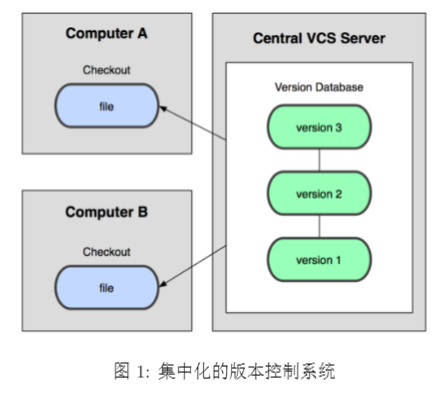
\includegraphics[width=0.5\textwidth]{images/insert-png.png} %插入图片,[]中设置图片大小,{}中是图片文件名
            \caption{插入图片的demo} %最终文档中希望显示的图片标题
            \label{Fig.insert-one-png} %用于文内引用的标签
        \end{figure}
    \end{lstlisting}

    \item 最终效果,图\ref{Fig.insert-one-png}
          \begin{figure}[H] %H为当前位置,!htb为忽略美学标准,htbp为浮动图形
              \centering %图片居中
              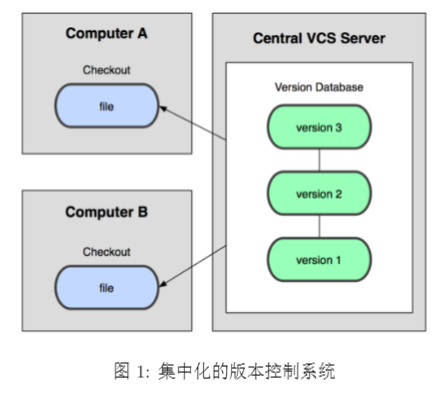
\includegraphics[width=0.5\textwidth]{images/insert-png.png} %插入图片,[]中设置图片大小,{}中是图片文件名
              \caption{插入图片的demo} %最终文档中希望显示的图片标题
              \label{Fig.insert-one-png} %用于文内引用的标签
          \end{figure}

    \item 双排设置
          \begin{lstlisting}
    Figure \ref{Fig.main} has two sub figures, fig. \ref{Fig.sub.1} is the travel demand of driving auto, and fig. \ref{Fig.sub.2} is the travel demand of park-and-ride.

    \begin{figure}[H]
    \centering  %图片全局居中
    \subfigure[name1]
    {
        \label{Fig.sub.1}
        \includegraphics[width=0.45\textwidth]{DV_demand}
    }
    \subfigure[name2]
    {
        \label{Fig.sub.2}
        \includegraphics[width=0.45\textwidth]{P+R_demand}
    }
    \caption{Main name}

    \label{Fig.main}
    \end{figure}
            \end{lstlisting}

    \item 双排效果显示,图 \ref{Fig.Insert_two_pic_demo}
          \begin{figure}[H]
              \centering
              %插入图片,[]中设置图片大小,{}中是图片文件名
              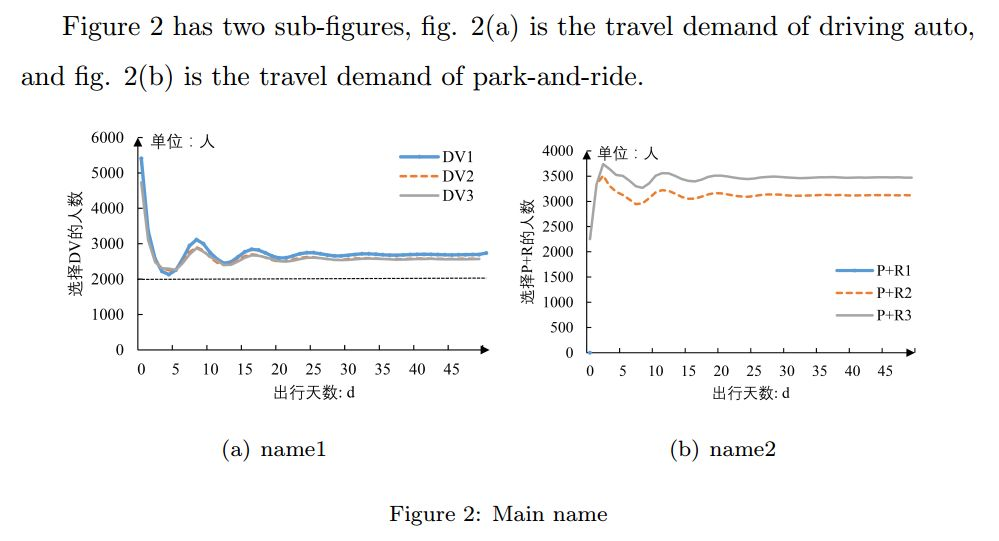
\includegraphics[width=1.0\textwidth]{images/insert-two-pic.jpg}
              \caption{并排插入两个图片的效果}
              \label{Fig.Insert_two_pic_demo}
          \end{figure}

    \item 引用图片

          在文档中使用$\backslash$ref\{标签\},如\verb!\ref{Fig.insert-one-png}!

\end{enumerate}








\subsection{如何设置边距}
\subsubsection{操作步骤}
\begin{enumerate}
    \item 引用geo 设置宏包
          $\backslash$usepackage\{geometry\}
    \item 设置页边距
          \begin{enumerate}
              \item 设置纸张大小,也可以设置常用的a4paper之类的。

                    \verb!\geometry{papersize={20cm,15cm}}!
              \item 设置为缩放的形式

                    \verb!\geometry{a4paper,scale=0.8}!
              \item 设置为绝对距离

                    \verb!\geometry\{a4paper,left=2cm,right=2cm,top=2cm,bottom=2cm\}!
          \end{enumerate}
    \item 效果不错

\end{enumerate}


\subsubsection{页面边距设置概念}

\begin{figure}[H] %H为当前位置,!htb为忽略美学标准,htbp为浮动图形
    \centering %图片居中
    %插入图片,[]中设置图片大小,{}中是图片文件名
    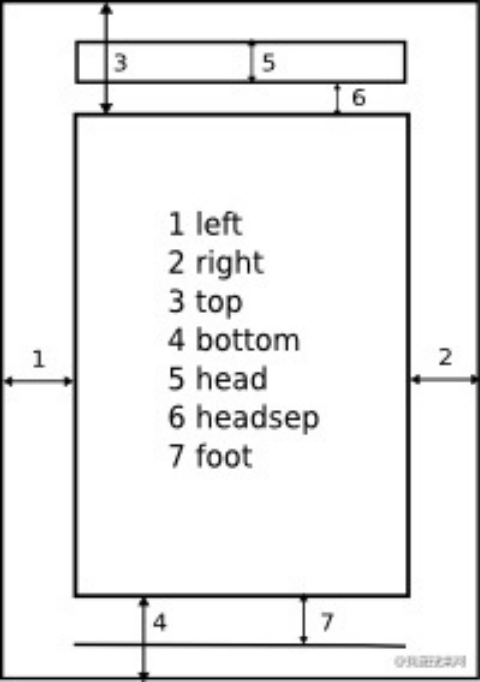
\includegraphics[scale=0.75]{images/geometry.png}
    \caption{页边距概念} %最终文档中希望显示的图片标题
    \label{Fig.page_border} %用于文内引用的标签
\end{figure}



\newpage
\section{\LaTeX 高级技巧}
\subsection{我们如何知道需要引用什么宏呢?}
当我们需要用什么东西的时候,我们该如何知道要引用什么?
比如我们要用超链接,我们就需要引用 hyperref 这个宏包?那我该如何知道呢?

知乎讨论: \href{https://www.zhihu.com/question/26421957}{用 TeX 编辑论文时,如何选择合适的 Packages ?}

CTAN (Comprehensive TeX Archive Network) 是干什么的,各位从它的名字应该能看出来。一般来说,如果有作者写了一个宏包,自觉还挺有价值,测试之后与常用宏包没有发现冲突,就会考虑上传到 CTAN 这个网站。CTAN 网站经过收集、整合、分类,给广大 TeX 用户提供了方便的检索系统:\href{http://www.ctan.org/ctan-portal/search/?ext=true/}{CTAN: Search}。 具体的用法可以参见页面当中的 Search Tips。

% \usepackage{bbding}
% \usepackage{pifont}
% \usepackage{wasysym}
% \usepackage{amssymb}


% amssymb
\checkmark

% bbding
\Checkmark
\CheckmarkBold

% pifont
\ding{51}
\ding{52}

% wasysym
\CheckedBox



%*如何对宏进行配置?
\subsection{如何对宏进行配置?}
当我们引用一个宏的时候,我们如何知道怎么配置这个宏呢?
比如我们引用 hyperref 宏的时候。我是如何知道我可以配置一下的这些东西呢?

\begin{lstlisting}
\hypersetup{
    colorlinks  = true,
    linkcolor   = blue,
    filecolor   = magenta,
    urlcolor    = cyan,
    % pdftitle    = {Overleaf Example},
    % pdfpagemode = FullScreen,
}
\end{lstlisting}



%*编译的过程
\subsection{\LaTeX 编译过程}
\label{subsec:buildprocess}
生成一个文档,需要使用排版软件进行编译生成,这就要涉及不同的步骤。

附带参考文献的整个编译需要四步。

\begin{lstlisting}
(xe/pdf)latex main.tex   # 表示使用 latex, pdflatex 或 xelatex 编译,下同
bibtex main.aux
(xe/pdf)latex main.tex
(xe/pdf)latex main.tex
\end{lstlisting}

第一步后生成main.aux、main.log和main.pdf文件。其中aux是引用标记记录文件,用于再次编译时生成参考文献和超链接。此时的pdf文件中没有包含参考文件,在正文中的引用后为[?]。

第二步后生成main.bbl和main.blg文件。blg为bibtex处理过程记录文件。

第三步后更新了main.aux、main.log和main.pdf文件。此时的pdf文件的末尾已经有了参考文献列表,但是在正文中的引用后仍然为[?]。

第四步同样更新了main.aux、main.log和main.pdf文件。并生成最终的pdf文件,此时正文中的引用后已经标记好了引用文献的序号[1]、[2]等。

如果对这个编译流程非常熟悉的话,就可以自己编写脚本快速编译了。当然还是推荐使用 VSCode\ref{subsec:recipe}。
\begin{lstlisting}
    @compile.bat文件

    @echo off
    set CompileName="pdflatex"
    for %%F in (*.tex) do (
    set FileName=%%~nF
    )
    if not exist "./Tmp" (
     md Tmp
     )

    %CompileName% -output-directory=Tmp %FileName%
    bibtex ./Tmp/%FileName%
    %CompileName% -output-directory=Tmp %FileName%
    %CompileName% -output-directory=Tmp %FileName%

    echo ------------------------------------------------
    echo Compile  finished.
    echo ------------------------------------------------
    copy /Y ".\Tmp\%FileName%.pdf" ".\%FileName%.pdf"
    start  " " /max "./%FileName%.pdf"
\end{lstlisting}



\subsection{什么是 recipe?}
\label{subsec:recipe}

\href{https://blog.csdn.net/qysh123/article/details/11833649}{PDFLaTeX和XeLaTeX有什么区别?}

\href{https://www.zhihu.com/question/31850346}{\LaTeX (\LaTeXe )写的文档如何一键转为word?}

通过上述编译流程\ref{subsec:buildprocess}, 对于简单的xeLaTeX 进行编译,只需要编译一次就够了。但是如果需要生成目录等文档,就需要使用xeLaTeX进行编译两次。如果还要使用bibTex 进行引用的话,还需要使用bibtex 进行编译,之后在用xeLaTeX进行编译两次。

对于不同的编译流程,就是所谓的 recipe。不同的文档类型有不同的编译流程。

因此我们需要根据自己的需求,自己定义这个编译流程。这也是\LaTeX 入手很难的原因之一。



\subsubsection{使用VSCode+\LaTeX \space WorkShop 进行编译}


一个 \LaTeX \space  recipe 是指在构建 \LaTeX \space 项目时,\LaTeX \space  Workshop 按顺序执行的一系列命令。它是由 latex-workshop.latex.recipes 定义的。默认情况下,\LaTeX \space  Workshop 包含由变量 latex-workshop.latex.recipes 和 latex-workshop.latex.tools 定义的两个基本 recipes。

\paragraph*{latex-workshop.latex.recipes}
用来定义编译流程。 您可以使用不同的工具创建多个 recipes。每个 recipe 都是配置列表中的一个对象,包含一个 name 字段和一个要在 recipe 中调用的 tools 列表。

\paragraph*{latex-workshop.latex.tools}
用来定义每个编译的参数。recipes 中的 tools 可以在 latex-workshop.latex.tools 中定义,其中每个命令都是一个 tool。每个工具都是一个对象,包括一个 name、要生成的一个 command、参数(args)和一些特定的环境变量(env)。env 条目是一个字典。假设您想要在您的home项目中使用一个 texmf 子目录,只需编写:

\begin{lstlisting}
"env": {
    "TEXMFHOME": "%DIR%/texmf"
}
\end{lstlisting}


\paragraph*{\LaTeX\space Workshop 参数}

对于命令里面的参数,可以查看下表\ref{tab.latex_args}:

\begin{table}[htbp]
    \centering
    \begin{tabular}{|c|l|}
        \hline
        占位符      & 替换为                                        \\
        \hline
        \%DOC\%     & LaTeX根文件路径和名称,不带.tex扩展名         \\
        \%DOCFILE\% & 不带.tex扩展名的LaTeX根文件名                 \\
        \%DIR\%     & LaTeX根文件路径                               \\
        \%TMPDIR\%  & 存储辅助文件的临时文件夹                      \\
        \%OUTDIR\%  & 在latex-workshop.latex.outDir中配置的输出目录 \\
        \hline
    \end{tabular}
    \caption{\LaTeX\space Workshop tool 参数占位符}
    \label{tab.latex_args}
\end{table}

\subsection{Lex, LaTex, pdflatex, xelatex, xetex等的区别和关系}

TeX:一种宏语言。

Plain Tex: Tex中的一个最基本的宏集合与TeX的基础语言构成的一种格式。

LaTex: Tex中的一个宏集合,构成一种与 Plain TeX 不一样的格式。

Tex程序:把Tex语言转换为排版的程序,也叫Tex。为区别,称这个 TeX 程序叫Knuth TeX。

tex命令:Tex程序中的编译命令。tex命令默认用Plain TeX格式进行排版。也就是说tex命令后面默认跟的tex文件应该是用Plain Tex格式写的。

latex命令:tex命令加上某一个选项使用,就会用LaTeX 格式进行排版,也就是说此时后面跟的tex文件应该是用LaTex格式写的。为方便,就把tex 命令与对应编译选项合成为一个命令,叫latex命令。

$\varepsilon$-TeX 程序:Knuth TeX程序的一个扩展,也是一个程序,一般写成 eTeX。增加了少量的几个命令,但一般来说是与Knuth TeX程序没有太多区别的。

\begin{quote}
    实现:在文中的意思就是指“程序”的意思。如文中:eTeX 程序和 Knuth TeX 都是TeX语言的一个实现(也就是说,eTeX 程序和 Knuth TeX 都是把TeX语言转换为排版的程序。程序作用于tex文本文件,把tex文件编译成dvi文件)。
\end{quote}

pdfTeX程序:Tex语言的又一个实现,也就是把Tex语言转换为排版的又一个程序。它会把 TeX 语言写的代码直接编译成 PDF 文件。

pdftex命令:pdfTex程序中的命令,用来编译用Plain TeX格式写的tex文件。

pdflatex命令:pdfTex程序中的命令,用来编译用LaTeX格式写的tex文件。

XeTeX程序:TeX语言的新的实现,即把Tex语言转换为排版的一个新程序。支持Unicode 编码和直接访问操作系统字体。

xetex命令:XeTeX程序中的命令,用来编译用Plain TeX格式写的tex文件。

xelatex命令:XeTeX程序中的命令,用来编译用LaTeX格式写的tex文件。

其中“实现”这个概念比较别扭,不知是不是计算机中的概念,反正非计算机专业的人读起来不知道“实现”是什么意思,不知道“TeX语言的一个实现”是什么意思。如果把“TeX语言的一个实现”写成是把TeX语言转换为排版的一个程序,这个程序作用于tex文本文件,把tex文件编译成某些文件,如dvi,pdf文件(比如pdfTex程序把tex文件编译成pdf文件)。那就好理解多了。

不知道上述理解对不对。如有错误,还请各位指点。

另外,我觉得,介绍概念时可以采用数学上的定义的方法,单独列出来每个概念的定义,每个概念的定义中不能含有前面没有定义的概念。这样就会让人好理解的多。上面我写的摘要就是这样做的。

\end{document}